\begin{figure}[H]
    \centering
    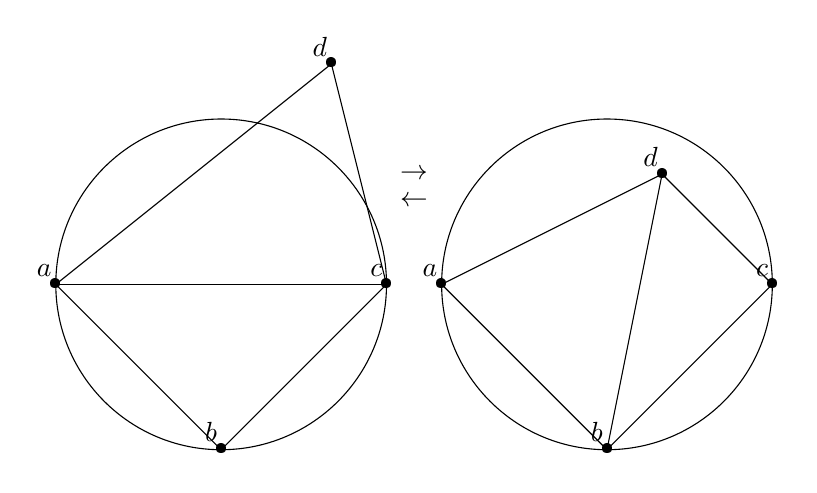
\begin{tikzpicture}[scale=0.7]
        \node[circle,draw,minimum size=4.2cm] at (0,0) {};
        \node[label={[label distance = -3mm]160:$a$}] at (-3.0, 0) {\textbullet};
        \node[label={[label distance = -3mm]160:$b$}] at (0, -3) {\textbullet};
        \node[label={[label distance = -3mm]160:$c$}] at (3, 0) {\textbullet};
        \node[label={[label distance = -3mm]160:$d$}] at (2, 4) {\textbullet};

        \draw (-3, 0) -- (0, -3);
        \draw (0, -3) -- (3, 0);
        \draw (-3, 0) -- (3, 0);
        \draw (-3, 0) -- (2, 4);
        \draw (2, 4) -- (3, 0);

        \node at (3.5, 2.00) {$\rightarrow$};
        \node at (3.5, 1.5) {$\leftarrow$};

        \begin{scope}
            [shift={(7, 0)}]
            \node[circle,draw,minimum size=4.2cm] at (0,0) {};
            \node[label={[label distance = -3mm]160:$a$}] at (-3.0, 0) {\textbullet};
            \node[label={[label distance = -3mm]160:$b$}] at (0, -3) {\textbullet};
            \node[label={[label distance = -3mm]160:$c$}] at (3, 0) {\textbullet};
            \node[label={[label distance = -3mm]160:$d$}] at (1, 2) {\textbullet};

            \draw (-3, 0) -- (0, -3);
            \draw (0, -3) -- (3, 0);
            \draw (1, 2) -- (0, -3);
            \draw (-3, 0) -- (1, 2);
            \draw (1, 2) -- (3, 0);
        \end{scope}

    \end{tikzpicture}
    \caption[Exemplo evento \textsc{incircle}]{Após a entrada de $d$ no círculo definido por $a$,
    $b$ e $c$, a aresta $ac$ se torna inválida e é trocada para uma aresta $bd$.}
    \label{fig:delaunay:incircle}
\end{figure}